\documentclass[10pt,a4paper]{article}
\usepackage[latin1]{inputenc}
\usepackage{amsmath}
\usepackage{amsfonts}
\usepackage{amssymb}
\usepackage{graphicx}
\usepackage[width=17.00cm, height=29.00cm]{geometry}
\author{Fabian Schubert}
\begin{document}
	\begin{figure}[h]
		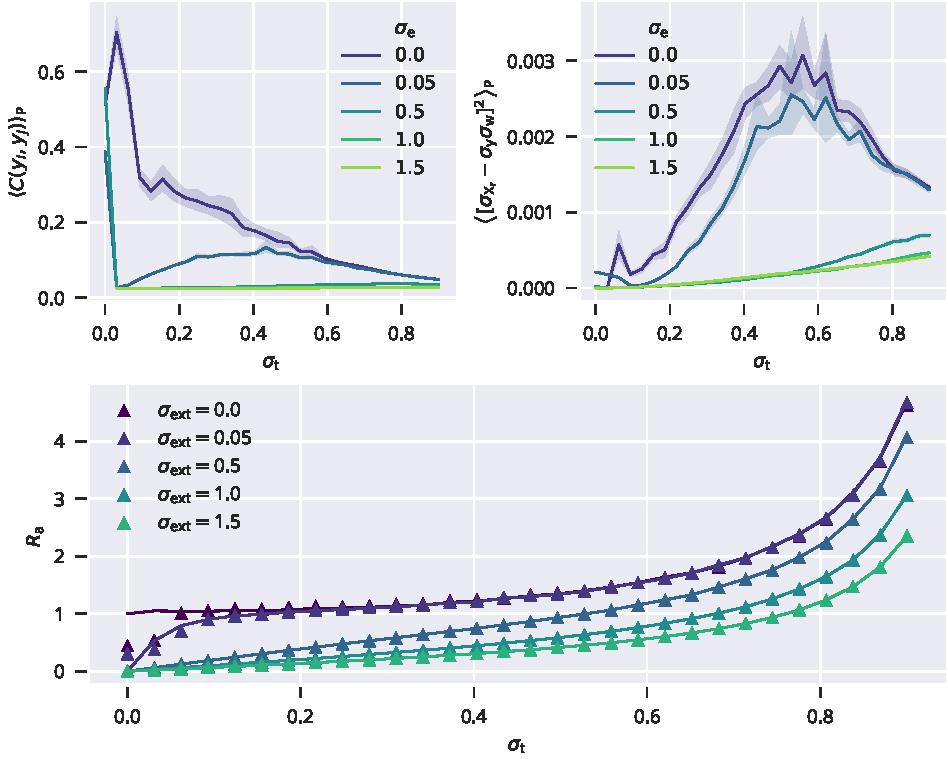
\includegraphics{../plots/homogeneous_independent_gaussian_input_compos.pdf}
		\caption{Homogeneous Independent Gaussian Input}
	\end{figure}
	\begin{figure}[h!]
		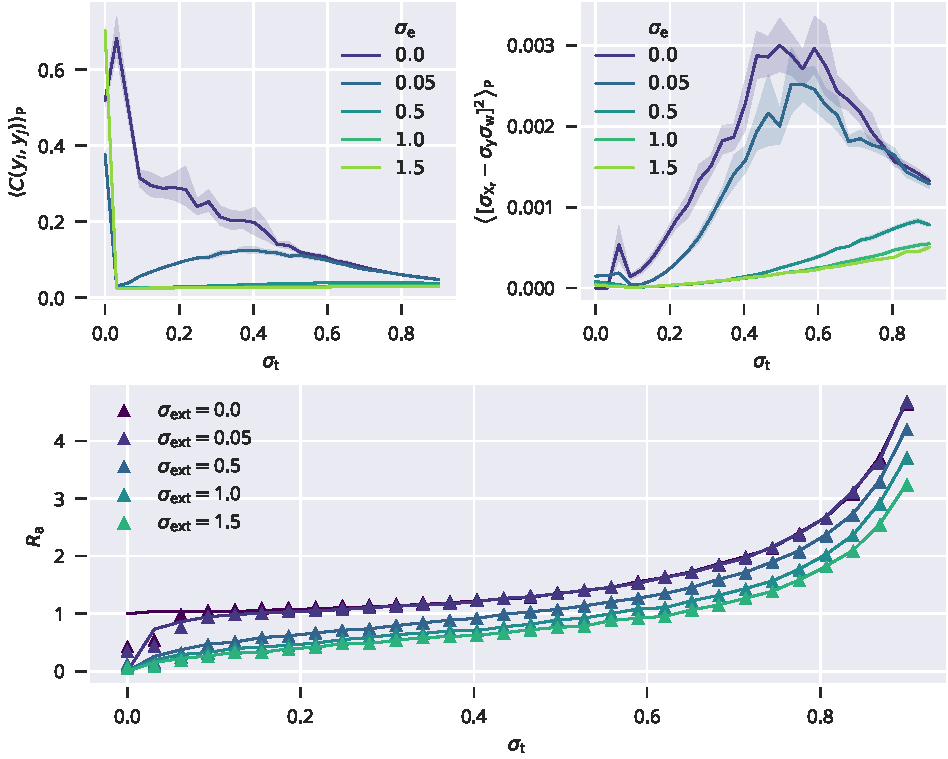
\includegraphics{../plots/heterogeneous_independent_gaussian_input_compos.pdf}
		\caption{Heterogeneous Independent Gaussian Input}
	\end{figure}
	\begin{figure}[h]
		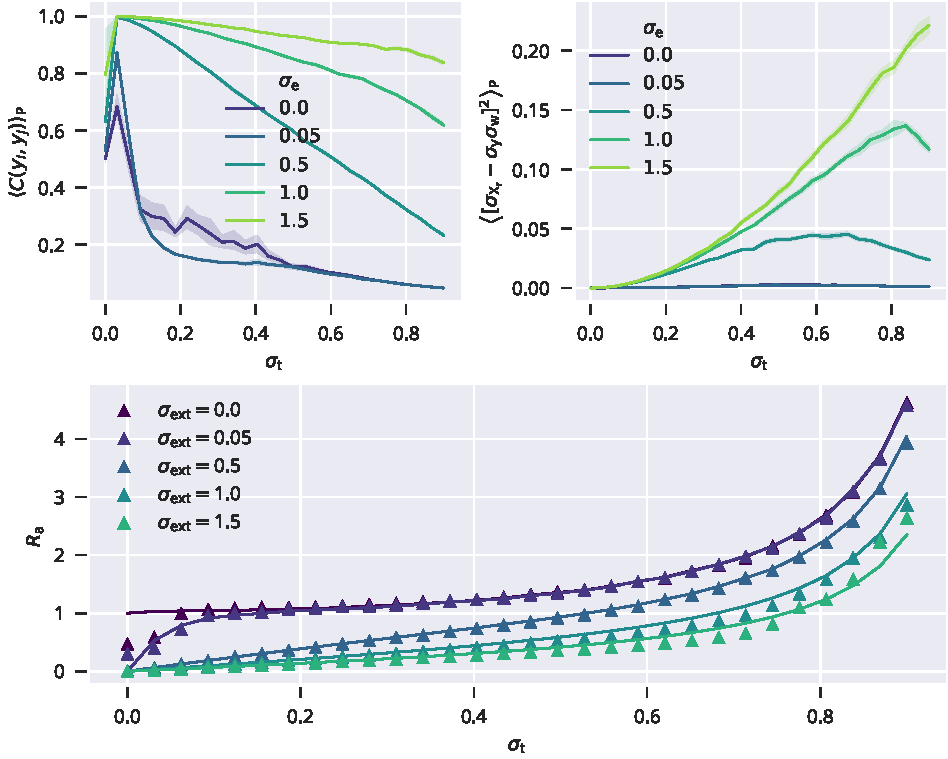
\includegraphics{../plots/homogeneous_identical_binary_input_compos.pdf}
		\caption{Homogeneous Identical Binary Input}
	\end{figure}
	\begin{figure}[h]
		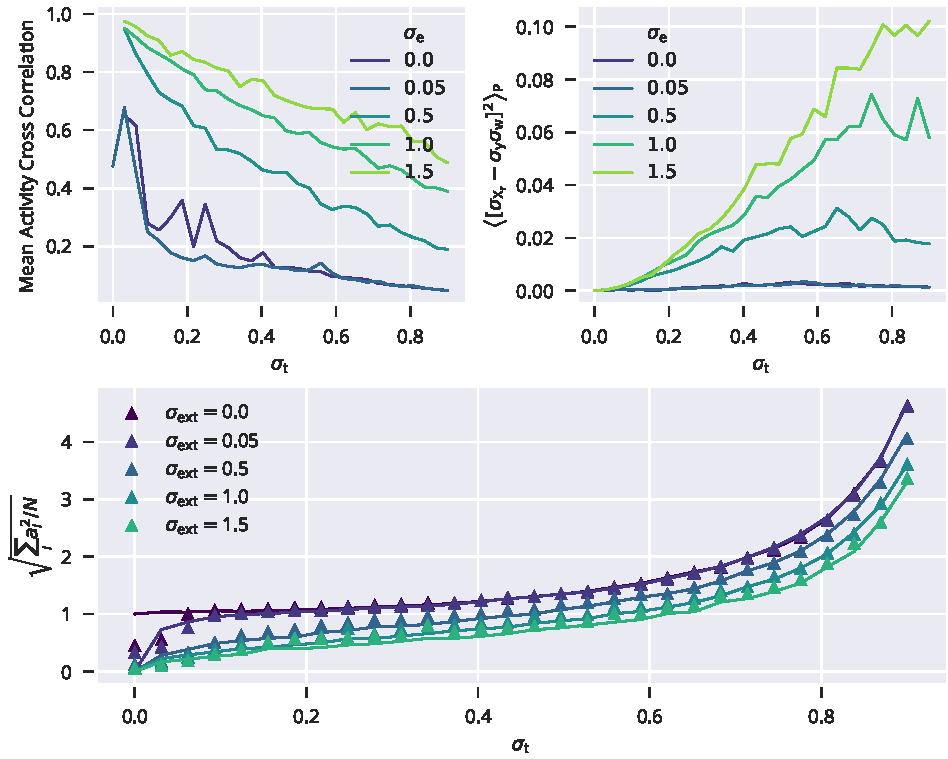
\includegraphics{../plots/heterogeneous_identical_binary_input_compos.pdf}
		\caption{Heterogeneous Identical Binary Input}
	\end{figure}
	\newpage
	\begin{figure}[h]
		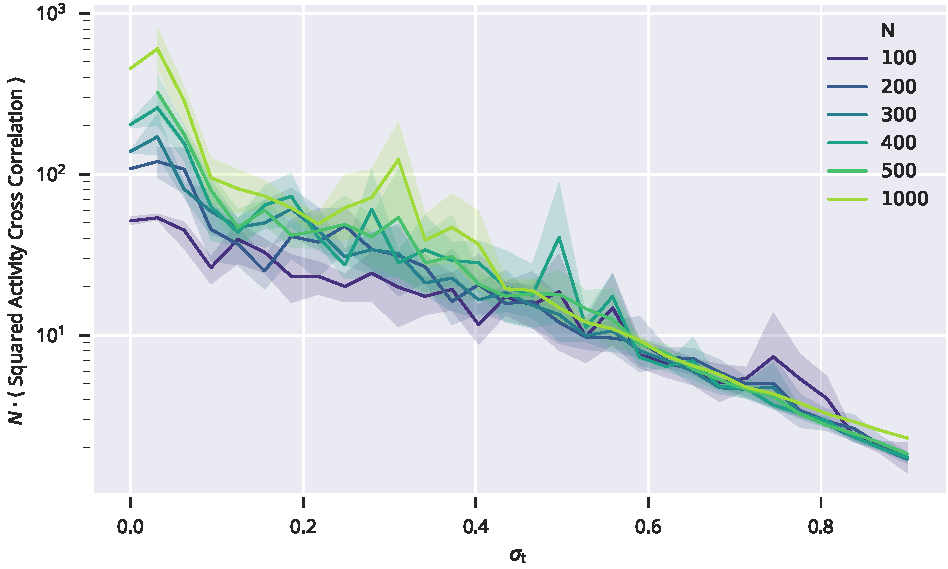
\includegraphics{../plots/homogeneous_independent_gaussian_input_corr_act_size_scaling_log.pdf}
		\caption{Autonomous System Correlation Scaling with Size}
	\end{figure}
	
	\begin{figure}[h]
		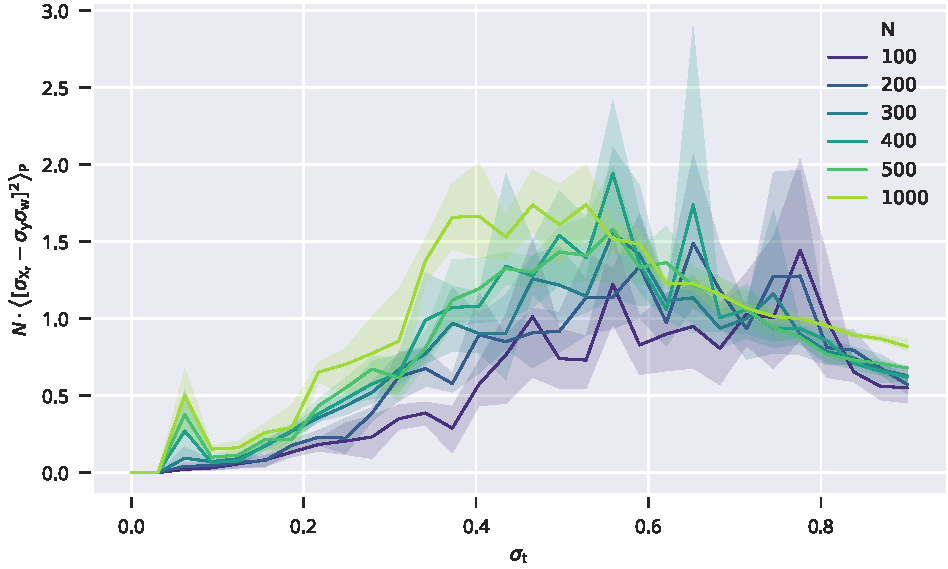
\includegraphics{../plots/homogeneous_independent_gaussian_input_rec_mem_pot_predict_size_scaling.pdf}
		\caption{Autonomous System Recurrent Variance Scaling with Size}
	\end{figure}



\end{document}